\documentclass[12pt]{amsart}

\usepackage{amsmath}
\usepackage{amssymb}
\usepackage{amsfonts}
\usepackage[alphabetic]{amsrefs}
\usepackage{amsthm}
\usepackage{enumitem}
\usepackage{fullpage}
\usepackage{color}
\usepackage{graphicx}

%%%%%%%%%%%%%% IMPORT QUIVER FOR COMMUTATIVE DIAGRAMS
% *** quiver ***
% A package for drawing commutative diagrams exported from https://q.uiver.app.
%
% This package is currently a wrapper around the `tikz-cd` package, importing necessary TikZ
% libraries, and defining a new TikZ style for curves of a fixed height.
%
% Version: 1.5.0
% Authors:
% - varkor (https://github.com/varkor)
% - AndréC (https://tex.stackexchange.com/users/138900/andr%C3%A9c)

\NeedsTeXFormat{LaTeX2e}
\ProvidesPackage{quiver}[2021/01/11 quiver]

% `tikz-cd` is necessary to draw commutative diagrams.
\RequirePackage{tikz-cd}
% `amssymb` is necessary for `\lrcorner` and `\ulcorner`.
\RequirePackage{amssymb}
% `calc` is necessary to draw curved arrows.
\usetikzlibrary{calc}
% `pathmorphing` is necessary to draw squiggly arrows.
\usetikzlibrary{decorations.pathmorphing}

% A TikZ style for curved arrows of a fixed height, due to AndréC.
\tikzset{curve/.style={settings={#1},to path={(\tikztostart)
    .. controls ($(\tikztostart)!\pv{pos}!(\tikztotarget)!\pv{height}!270:(\tikztotarget)$)
    and ($(\tikztostart)!1-\pv{pos}!(\tikztotarget)!\pv{height}!270:(\tikztotarget)$)
    .. (\tikztotarget)\tikztonodes}},
    settings/.code={\tikzset{quiver/.cd,#1}
        \def\pv##1{\pgfkeysvalueof{/tikz/quiver/##1}}},
    quiver/.cd,pos/.initial=0.35,height/.initial=0}

% TikZ arrowhead/tail styles.
\tikzset{tail reversed/.code={\pgfsetarrowsstart{tikzcd to}}}
\tikzset{2tail/.code={\pgfsetarrowsstart{Implies[reversed]}}}
\tikzset{2tail reversed/.code={\pgfsetarrowsstart{Implies}}}
% TikZ arrow styles.
\tikzset{no body/.style={/tikz/dash pattern=on 0 off 1mm}}

\newcommand{\An}{\mathbb{A}^n}
\newcommand{\Pn}{\mathbb{P}^n}
\renewcommand{\a}{\mathfrak{a}}
\newcommand{\C}{\mathbb{C}}
\newcommand{\Z}{\mathbb{Z}}
\newcommand{\Q}{\mathbb{Q}}
\newcommand{\g}{\mathfrak{g}}
\newcommand{\h}{\mathfrak{h}}
\newcommand{\ad}{\mathrm{ad}}
\newcommand{\git}{/\!\!/}

\newtheorem{theorem}{Theorem}[subsection]
\newtheorem{definition}[theorem]{Definition}
\newtheorem{corollary}[theorem]{Corollary}
\newtheorem{lemma}[theorem]{Lemma}
\newtheorem*{exercise}{Exercise}
\newtheorem{proposition}[theorem]{Proposition}
\newtheorem{claim}[theorem]{Claim}

\theoremstyle{remark}
\newtheorem*{remark}{Remark}

\theoremstyle{remark}
\newtheorem*{example}{Example}

\theoremstyle{remark}
\newtheorem*{moreexamples}{More examples}

\allowdisplaybreaks

\title{Honours Project}
\author{Declan Fletcher}
\date{}

\begin{document}

\maketitle

\tableofcontents

\section{Algebraic varieties}
\subsection{Affine varieties}
Affine $n$-space over $k$, denoted $\An_k$ or simply $\An$, is the set of $n$-tuples of elements of $k$, i.e.,
$$\An = \{(a_1, \dots, a_n) \, : \, a_i \in k\}.$$
Elements of $\An$ are called points, and if $P = (a_1, \dots, a_n)$ then the $a_i$ are called the coordinates of $P$.
Let $A = k[x_1, \dots, x_n]$ be the polynomial ring in $n$ variables over $k$, which we interpret as the ring of polynomial functions on $\An$ by defining $f(P) = f(a_1, \dots, a_n)$ for $P \in \An$ and $f \in A$.
This allows us to talk about the zeros of a polynomial $f$, namely 
$$Z(f) = \{P \in \An \, : \, f(P) = 0\}.$$
More generally, if $T$ is any set of polynomials (i.e., $T \subseteq A$), we define the zero set of $T$ as the points where all polynomials in $T$ vanish, meaning 
$$Z(T) = \{P \in \An \, : \, f(P) = 0 \text{ for all } f \in T\}.$$
Note that if $\mathfrak{a}$ is the ideal generated by $T$, then $Z(\mathfrak{a}) = Z(T)$. 
Since $A$ is a Noetherian ring (to do: prove this  --- ``Hilbert's basis theorem''), any ideal has a finite set of generators $f_1, \dots, f_r$ and $Z(T)$ can be expressed as $Z(\{f_1, \dots, f_r\})$.

\begin{definition}
A subset $Y \subseteq \An$ is called algebraic if $Y$ is the set of common zeros of a set of polynomials, i.e., if there exists $T \subseteq A$ such that $Y = Z(T)$.
\end{definition}

\begin{example}
Any line in $\mathbb{A}^2$ is the set of zeros of the polynomial $ax + by - c$ for some $a, b, c \in k$.
Therefore lines are algebraic.
The parabola $Z(\{y - x^2\})$ is an algebraic set.
\end{example}

\begin{proposition}[{\cite[Prop 1.1]{Hartshorne77}}]
We have the following properties of algebraic sets:
\begin{enumerate}
\item
If $Y_1$ and $Y_2$ are algebraic sets , then $Y_1 \cup Y_2$ is an algebraic set.

\item
If $\{Y_i\}_{i \in I}$ is an arbitrary collection of algebraic sets, then $\bigcap_{i \in I} Y_i$ is algebraic.

\item
$\emptyset$ and $\An$ are algebraic sets.
\end{enumerate}
\end{proposition}
\begin{proof}
(1) Suppose $Y_1 = Z(T_1)$ and $Y_2 = Z(T_2)$ where $T_1, T_2 \subseteq A$.
We claim that $Y_1 \cup Y_2 = Z(T_1 T_2)$, where $T_1 T_2 = \{f g \, : \, f \in T_1, g \in T_2\}$.
If $P \in Y_1 \cup Y_2$, assume without loss of generality that $P \in Y_1$.
Then for all $f \in T_1$, $f(P) = 0$, and $(fg)(P) = 0$ for all $fg \in T_1 T_2$ so $P \in Z(T_1 T_2)$.
Let $P \in Z(T_1 T_2)$.
If $f(P) = 0$ for all $f \in T_1$, then $P \in Z(T_1) = Y_1$.
Otherwise, let $f \in T_1$ such that $f(P) \ne 0$.
Since $P \in Z(T_1 T_2)$, we have $(fg)(P) = 0$ which implies $g(P) = 0$ for all all $g \in T_2$.
This means $P \in Z(T_2) = Y_2$ and in either case $P \in Y_1 \cup Y_2$.

(2) Let $\{Y_i\}_{i \in I}$ be algebraic sets such that $Y_i = Z(T_i)$ for each $i$.
Then
$$\bigcap_{i \in I} Y_i = \bigcap_{i \in I} Z(T_i) = \{P \in \An \, : \, f(P) = 0 \text{ for all } f  \in T_i, \text{ for all } i \in I\} = Z\left( \bigcup_{i \in I} T_i\right).$$

(3) Note that $\emptyset = Z(\{1\})$ and $\An = Z(\{0\})$.
\end{proof}

\begin{example}
The lines $y - x = 0$ and $y + x = 0$ are algebraic, and their union is defined by $y^2 - x^2 = (y-x)(y+x) = 0$.
If $\{Y_a\}_{a \in k}$, where each $Y_a = Z(\{y=ax\})$, is the set of lines through the origin, then $\bigcap Y_a = Z \left(\bigcup Y_a\right) = \{(0, 0)\}$.
Therefore $\{(0, 0)\}$ is an algebraic set in $\mathbb{A}^2$. 
\end{example}

\begin{definition}[Zariski topology]
The Zariski topology is on $\An$ is defined by taking the open subsets to be the complements of the algebraic sets, i.e., the algebraic sets are the closed sets.
The previous proposition implies this satisfies the axioms for a topology.
\end{definition}

\begin{example}[The Zariski topology on $\mathbb{A}^1$]
Let $Z(T)$ be an algebraic set where $T \subseteq A = k[x]$.
Since $Z(T) = Z(\mathfrak{a})$ for $\mathfrak{a} = \langle T \rangle$, and every ideal in $k[x]$ is principal ($k[x]$ is a PID since it is a Euclidean domain), $Z(T) = Z(\{f\})$ for some $f \in A$.
So every algebraic set in $\mathbb{A}^1$ is the zero set of a single polynomial.
Further, since $k$ is algebraic closed, any nonconstant $f$ can be written $f = c(x - a_1) \dots (x-a_n)$ for some $c, a_i \in k$.
So $Z(T) = Z(\{f\}) = \{a_1, \ldots, a_n\}$, meaning we can conclude every algebraic set in $\mathbb{A}^1$ is simply a finite set of points (or $\emptyset$ or $\mathbb{A}^1$).
Correspondingly, the open sets are $\emptyset$, $\mathbb{A}^1$, and the complements of finite sets.
Note this implies the Zariski topology is not Hausdorff;
if we try to find open sets $U$ and $V$ that separate the points, say, $0$ and $1$, $U$ and $V$ will contain an infinite number of points and must necessarily intersect.
\end{example}

\begin{definition}[Irreducible set]
A nonempty subset $Y$ of a topological space $X$ is irreducible if it cannot be expressed as the union $Y = Y_1 \cup Y_2$ of two proper subsets which are each closed in $Y$.
The empty set is not considered to be irreducible.
\end{definition}

\begin{example}
$\mathbb{A}^1$ is irreducible because its only proper subsets are finite yet it is infinite ($k$ is necessarily infinite since it is algebraically closed).
The algebraic set $Z(y^2 - x^2)$ is reducible since $Z(y^2 - x^2) = Z(y - x) \cup Z(y +x)$.
\end{example}

\begin{definition}[Affine algebraic variety]
An affine algebraic variety (or simply affine variety) is an irreducible closed subset on $\An$ with the induced topology.
An open subset of an affine variety is a quasi-affine variety.
\end{definition}

Affine and quasi-affine varieties are the first objects of study in algebraic geometry.
However, the study of these objects rely deeply on the relationship between subsets of $\An$ and ideals in $A$, so we need to investigate this relationship further (this will help us give examples of affine varieties).
For a subset $Y \subseteq \An$, define the ideal of $Y$ in $A$ by
$$I(Y) = \{f \in A \, : \, f(P) = 0 \text{ for all } P \in Y\}.$$
Now we have the function $Z$ which maps subsets of $A$ to algebraic sets, and $I$ which maps subsets of $\An$ to ideals.

Establishing the connection between ideals and sets relies on Hilbert's famous \emph{Nullstellensatz}:

\begin{theorem}[Hilbert's Nullstellensatz]
Let $k$ be an algebraically closed field, let $\a$ be an ideal in $A = k[x_1, \dots, x_n]$, and let $f \in A$ be a polynomial which vanishes at all points of $Z(\a)$.
Then $f^r \in \a$ for some integer $r > 0$.
\end{theorem}

This implies the following:

\begin{proposition}[{\cite[Prop 1.2]{Hartshorne77}}]
We have the following propeties of $Z$ and $I$:
\begin{enumerate}[label=(\roman*)]
\item
If $T_1 \subseteq T_2$ are subsets of $A$, then $Z(T_1) \supseteq Z(T_2)$.

\item
If $Y_1 \subseteq Y_2$ are subsets of $\An$, then $I(Y_1) \supseteq I(Y_2)$.

\item
For any two subsets $Y_1, Y_2 \subseteq \An$, we have $I(Y_1 \cup Y_2) = I(Y_1) \cap I(Y_2)$.

\item
For any ideal $\a \subseteq A$, $I(Z(\a)) = \sqrt{\a}$, the radical of $\a$.

\item
For any subset $Y \subseteq \An$, $Z(I(Y)) = \bar Y$, the (Zariski) closure of $Y$.
\end{enumerate}
\end{proposition}
\begin{proof}
(i) If all polynomials in $T_2$ vanish at $P$, then in particular all polynomials in $T_1$ vanish at $P$.

(ii) If $f$ is polynomial which vanishes at all $P \in Y_2$, then in particular $f$ vanishes at all $P \in Y_1$.

(iii) to do: complete this.
\end{proof}

\begin{corollary}[{\cite[Coro 1.4]{Hartshorne77}}]
There is a one-to-one inclusion-reversing correspondence between algebraic sets in $\An$ and radical ideals (i.e., ideals which are equal to their own radical) in $A$, given by $Y \mapsto I(Y)$ and $\a \mapsto Z(\a)$.
Furthermore, an algebraic set is irreducible if and only if its ideal is prime.
\end{corollary}
\begin{proof}
The first sentence is a direct consequence of (i), (ii), (iv) and (v) in the previous proposition.
Suppose $Y$ is irreducible.

\end{proof}

\begin{example}
This allows us to see $y = x^2$ is irreducible.
\end{example}

\begin{definition}[Affine coordinate ring]
If $Y \subseteq \An$ is an affine algebraic set, we define the affine coordinate ring of $Y$, denoted $A(Y)$, to be $A/I(Y)$.
\end{definition}

\begin{example}
The condition that an algebraic variety be irreducible implies $A(Y)$ is an integral domain.
To do: add an example and a counter-example.
\end{example}

\begin{example}
Coordinate ring of a line is $k[x]$.
\end{example}

\subsection{Projective varieties}
Projective varieties are similar to affine varieties, but are instead subsets of \emph{projective space}.
Projective space is the set of lines in an affine space.
Formally, projective $n$-space over $k$, denoted $\Pn_k$ or $\Pn$, is
$$\Pn = \{(a_0, \ldots, a_n) \ne (0, \ldots, 0) \, : \, a_i \in k \} / \sim$$
where
$$(a_0, \ldots, a_n) \sim (\lambda a_0, \ldots, \lambda a_n)$$
for all $\lambda \in k \setminus \{0\}$.
In other words, $\Pn$ is $\mathbb{A}^{n+1} \setminus \{(0, \ldots, 0)\}$ where lines lying on the same line through the origin are identified.

%\section{Reductive groups}
%
%\section{Lie algebras}
%
%\section{GIT and the Hilbert-Mumford Criterion}
%
%\section{The adjoint quotient}

\section{Chevalley's restriction theorem}
In this section, we will study Chevalley's restriction theorem, which elucidates the structure of $\C[\g]^G$.
To understand the statement, we require some preliminaries.
All facts in this section can be found in \cite{Humphreys72}.

\subsection{The Weyl group of $\g$}
Assume that $\g$ is a non-zero semisimple Lie algebra.
If $\h$ is a Cartan subalgebra and $\Phi$ is the corresponding root system, recall the root-space decomposition
$$\g = \h \oplus \bigoplus_{\alpha \in \Phi} \g_\alpha.$$
We have that if $x \in \g_\alpha$ for $\alpha \in \Phi$, $\ad_x$ is nilpotent.

Since $\g$ is semisimple, the Killing form restricted to $\h$ is non-degenerate, giving an identification between $\h$ and $\h^*$.
Specifically, $\phi \in \h^*$ corresponds to the unique $t_\alpha \in \h$ such that $\phi(h) = \kappa(t_\phi, h)$ for all $h \in \h$.
Since $\Phi$ is a spans $\h^*$, we have the corresponding spanning set for $\h$:
$$\Phi \subseteq \h^* \longleftrightarrow \{t_\alpha \, | \, \alpha \in \Phi\}$$
This identification induces an inner product on $\h^*$, given by
$$(\phi, \psi) = \kappa(t_\phi, t_\psi).$$

For any non-zero vector $\alpha \in \h^*$, we have a corresponding \emph{reflection}, $\sigma_\alpha$, defined by
$$\sigma_\alpha(\beta) = \beta - \frac{2 (\beta, \alpha)}{(\alpha, \alpha)} \alpha.$$
We note that this is a linear map sending $\alpha$ to $-\alpha$ and fixing pointwise the reflecting hyperplane $P_\alpha = \{\beta \in \h^*\, | \, (\alpha, \beta)=0\}.$

The \emph{Weyl group} of $\g$, $W$, is defined to be the group generated by all reflections $\sigma_\alpha$ with $\alpha \in \Phi$, i.e.,
$$W =\langle \sigma_\alpha \, | \, \alpha \in \Phi \rangle \subseteq GL(\h^*).$$
Since $\Phi$ is an abstract root system (see \cite[\S 9.2]{Humphreys72}), each reflection $\sigma_\alpha$ permutes $\Phi$.
Then $W$ is contained in the symmetric group on $\Phi$, implying it is finite.

\subsection{Inner automorphisms of $\g$}
Recall that an \emph{automorphism} of $\g$ is a Lie algebra isomorphism $\g \to \g$.

\begin{example}
If $\g \subseteq \mathfrak{gl}(V)$ and $a \in GL(V)$ such that $a \g a^{-1} = \g$, it is straightforward to check that the conjugation map $x \mapsto a x a^{-1}$ preserves the commutator, implying the map is an automorphism of $\g$.
\end{example}

If $x \in \g$ and $\ad_x$ is nilpotent, say $(\ad_x)^k = 0$, we can define $\exp(\ad_x)$ using the usual power series definition, which terminates by nilpotence:
$$\exp(\ad_x) = 1 + \ad_x + \frac{1}{2!} (\ad_x)^2 + \ldots + \frac{1}{(k-1)!} (\ad_x)^{k-1}.$$
It turns out that $\exp(\ad_x)$ will be an automorphism of $\g$, (see \cite[\S 2.3]{Humphreys72} for the computation).
We define 
$$\mathrm{Int}(\g) := \langle \exp(\ad_x) \, | \, x \in \g \text{ is nilpotent}\rangle,$$
the \emph{inner automorphisms}.
One can prove that the inner automorphisms form a normal subgroup of the group of automorphisms of $\g$ (again see \cite[\S 2.3]{Humphreys72}).

\begin{example}
Let $\g = \mathfrak{sl}_2(\C)$, with standard basis $\{e, h, f\}$.
A key example of an inner automorphism, which will be important for us later, is
$$\sigma = \exp(\ad_e)\exp(\ad_{-f})\exp(\ad_e).$$
A straightforward computation shows that $\sigma$ acts on the basis by
$$\sigma(e) = -f, \quad \sigma(f) = -e, \quad \sigma(h) = -h.$$
Consider the usual matrix exponentials 
$$\exp(e) = 
\begin{pmatrix}
	1 & 1 \\
	0 & 1 
\end{pmatrix},
\quad
\exp(-f) =
\begin{pmatrix}
	1 & 0 \\
	-1 & 1
\end{pmatrix},$$
which converge since $e, f$ are nilpotent matrices.
If
$$s = \exp(e) \exp(-y) \exp(e) =
\begin{pmatrix}
	0 & -1 \\
	1 & 1
\end{pmatrix},$$
we get that
$$s e s^{-1} = -f, \quad s f s^{-1} = -e, \quad s h e^{-1}=h,$$
so conjugation by $s$ acts in the same way as $\sigma$.
The general phenomena is:
if $\g \subseteq \mathfrak{gl}(V)$ and $x \in \g$ is nilpotent, then
$$\exp(x) y \exp(x)^{-1} = \exp(\ad_x)(y).$$
This means that if $\exp(\ad_x)$ is a generator for $\mathrm{Int}(\g)$, $\exp(x) \in G$ (here $G$ is the algebraic group that has $\g$ as it's Lie algebra) and then $\exp(\ad_x) \in \mathrm{Ad}(G)$.
So $\mathrm{Int}(\g) \subseteq \mathrm{Ad}(G)$.
%%%%%%%%%%%%%
%\textcolor{red}{Question: in Humphrey's book the statement $\C[\g]^G \cong \C[\h]^W$ takes $G = \mathrm{Int}(\g)$, but for our purposes we want $G$ to be an algebraic group acting on $\g$ by the adjoint action.
%Then one hopes these are the same thing, i.e., $\mathrm{Int}(\g) = \mathrm{Ad}(G)$ as a subgroup of $\mathrm{Aut}(\g)$.
%Is it clear why this is this case, or do we need some assumptions on $G$ for this to hold? 
%I think it's enough if $G$ is generated by elements $\exp(x)$ for $x \in \g$ nilpotent.}
\end{example}

It is necessary for Chevalley's restriction theorem to realise elements of the Weyl group as inner automorphisms.
(Generally, an automorphism of $\Phi$ determines an automorphism of $\h$, which can be extended to $\g$.)
We want to find an inner automorphism $\tau_\alpha$ that restricted to $\h$ acts like the reflection $\sigma_\alpha$.
For any non-zero $x_\alpha \in \g_\alpha$ for $\alpha \in \Delta$, let $y_\alpha \in h_\alpha$ satisfy $[x_\alpha, y_\alpha]=h_\alpha$.
We claim that 
$$\tau_\alpha = \exp(\ad_{x_\alpha})\exp(\ad_{-y_\alpha})\exp(\ad_{x_\alpha})$$
acts like $\sigma_\alpha$ on $\h$.
The previous example tells us that
$$\tau_\alpha(x_\alpha) = - y_\alpha, \quad \tau_\alpha(y_\alpha) = - x_\alpha, \quad \tau_\alpha(h_\alpha) = -h_\alpha.$$
We have $\h = \ker \alpha \oplus \mathrm{span} \{h_\alpha\}$.
If $h \in \ker \alpha$, 
$$\ad_{x_\alpha}(h) = [x_\alpha, h] = - \alpha(h) x_\alpha = 0,\quad \ad_{-y_\alpha}(h) = [-y_\alpha, h] = \alpha(h) y_\alpha =0,$$
so we readily see that $\tau_\alpha(h) = h$ for all $h \in \ker \alpha$.
This shows $\tau_\alpha$ agrees with the reflection $\sigma_\alpha$ on $\h$.
In this way, we realise generators (and therefore all elements) of the Weyl group as elements of $\mathrm{Int}(\g)$.
However, Humphreys \cite[\S 14.3]{Humphreys72} notes that the subgroup of $\mathrm{Int}(\g)$ generated by the $\tau_\alpha$, $\alpha \in \Delta$ may be bigger than the Weyl, so the Weyl group is not necessarily a subgroup of $\mathrm{Int}(\g)$.

\subsection{The symmetric algebra}
Let $V$ be any vector space over a field $k$.
The \emph{symmetric algebra on $V$}, $S(V)$, is defined as
$$S(V) = T(V) /\langle x \oplus y - y \oplus x \, | \, x, y \in V\rangle.$$
$S(V)$ enjoys the following universal property:
if $A$ is a commutative algebra, for any linear map $f: V \to A$, there exists a unique algebra homomorphism $g: S(V) \to A$ such that the following diagram commutes:
% https://q.uiver.app/#q=WzAsMyxbMCwwLCJWIl0sWzEsMCwiUyhWKSJdLFsxLDEsIkEiXSxbMCwxLCJcXGlvdGEiXSxbMSwyLCJnIl0sWzAsMiwiZiIsMl1d
\[\begin{tikzcd}
	V & {S(V)} \\
	& A
	\arrow["\iota", from=1-1, to=1-2]
	\arrow["g", from=1-2, to=2-2]
	\arrow["f"', from=1-1, to=2-2]
\end{tikzcd}\]
If $B$ is a basis for $V$, then $S(V)$ can be identified with $k[B]$ through a canonical isomorphism.
In this way, $S(V)$ can be thought of as a ``coordinate-free'' polynomial ring.

In stating Chevalley's restriction theorem, we will consider $S(\g^*)$ to be algebra of polynomial functions on $\g$.
If $G$ acts on $\g$, it acts on $S(\g^*)$ by
$$g \cdot (e_1 \otimes \ldots \otimes e_m) = (g\cdot e_1) \otimes \ldots \otimes (g \cdot e_m),$$
where $g \in G$ acts on $e_i \in V^*$ in the usual way that an action of a group on a vector space gives an action on the functions on that vector space:
$$(g\cdot e_i)(v) = e_i(g^{-1} \cdot v).$$

\subsection{Statement of the theorem}
Let $G = \mathrm{Int}(\g)$, which acts on $\g$.
Identify $\C[\g]$ with $S(\g^*)$, which has a natural action of $G$.
The polynomials fixed by the $G$ action are called the $G$-invariant polynomials, which is denoted $\C[\g]^G$; this space is identified with $S(\g^*)^G$.
Since we have realised the elements of $W$ as inner automorphisms, we have an action of $W$ on $\h$ and hence $\C[\h] \cong S(\h^*)$.
Therefore, we can also also consider the $W$-invariant polynomials on $\h$, $\C[\h]^W \cong S(\h^*)^W$.

Any polynomial function on $\g$ restricts to a polynomial function on $\h$ (this is clear if we extend a basis of $\h$ to a basis of $\g$, and think of polynomial functions on $\g$ as polynomials in the dual basis).
If $p \in \C[\g]^G$, in particular, $p$ is invariant under the action of the inner automorphisms $\tau_\alpha$, $\alpha \in \Delta$.
As $\left. \tau_\alpha \right|_\h$ is the reflection $\sigma_\alpha$, $\left. p \right|_\h$ is invariant under the generators of the Weyl group, so $\left. p \right|_\h \in \C[\h]^W$.
This implies that the restriction of polynomials map $\C[\g] \to \C[\h]$, $p \mapsto \left. p \right|_\h$, induces an algebra homomorphism
$$\theta: \C[\g]^G \to \C[\h]^W.$$
Chevalley's restriction theorem says that \emph{$\theta$ is an isomorphism}.

\begin{example}
Let's consider the case when $\g = \mathfrak{sl}_3(\C)$.
To explicitly see $\C[\g]^G$, we will use the fact that this ring of invariants is generated by the coefficents of the characteristic polynomial.
Noting that
$$
\begin{pmatrix}
	h_1 & a & b \\
	x & h_2 - h_1 & c \\
	y & z & - h_2
\end{pmatrix} \in \g$$
has characteristic polynomial
$$- \lambda^3 + (ax + by + cz + h_1^2 - h_1 h_2 + h_2^2) \lambda 
+( acy + ah_2x + bh_1y - bh_2y + bxz + ch_1z + h_1^2h_2 - h_1h_2^2),$$
under the restiction map $\C[\g] \to \C[\h]$, the generators of $\C[\g]^G$ map to 
\begin{align*}
	(ax + by + cz + h_1^2 - h_1 h_2 + h_2^2) &\mapsto h_1^2 - h_1 h_2 + h_2^2, \\
	(acy + ah_2x + bh_1y - bh_2y + bxz + ch_1z + h_1^2h_2 - h_1h_2^2) &\mapsto h_1^2 h_2 - h_1 h_2^2.
\end{align*}
Chevalley's restriction theorem tells us that
$$\C[\g]^G \cong \C[\h]^W = \C[h_1^2 - h_1 h_2 + h_2^2, h_1^2 h_2 - h_1 h_2^2].$$
%%%%%%%%%%%
%\textcolor{red}{
%I'm not sure that this seems correct.
%As I have written it in previous sections, the actions of the simple reflections should be $h_1 \mapsto - h_1$ and $h_2 \mapsto - h_2$.
%I don't think $\C[h_1^2 - h_1 h_2 + h_2^2, h_1^2 h_2 - h_1 h_2^2]$ is invariant under this action.
%The Weyl group should be $S_3$, but I don't see how this looks like permutations.
%}
\end{example}

\subsection{The adjoint quotient $\g\git G$}
The real goal of study Chevalley's restriction theorem is to understand $\g \git G$.
We have that 
$$\C[\g]^G \cong \C[\h]^W.$$
Another theorem, the Chevalley-Shephard-Todd theorem, implies that
$$\C[\h]^W \cong \C[x_1, \ldots, x_r],$$
where $r = \mathrm{rank}(T)$.
Therefore, 
$$\g \git G = \mathrm{Spec}(\C[\g]^G) \cong \mathrm{Spec}(\C[x_1, \ldots, x_r]) = \C^r.$$

We can also use the isomorphism $\C[\g]^G \cong \C[\h]^W$ to investigate the stability of $v \in \g$.
One formulation of stability says that $v \in \g$ is unstable if and only if for all $p \in \C[\g]^G$, $p(v) = p(0)$.
%%%%%%%%%%%
%\textcolor{red}{
%Ideally, we would be able to use the isomorphism to say that $v \in \g$ is unstable if and only if $\tilde p(0) = \tilde p(\left. v \right|_\h)$ for all $\tilde p \in \C[\h]^W$, though I'm not sure how to get this to work.
%If $v$ is unstable, for any $p \in \C[\g]^G$, $p(0) = p(v)$, so under the restriction map $p \mapsto \tilde p = \left. p \right|_\h$, we will get $\tilde p (0) = \tilde p (\left. v \right|_\h).$
%Conversely, for any $\tilde p \in \C[\h]^W$, there is a unique $p \in \C[\g]^G$ such that $\left. p \right|_\h = \tilde p$.
%Suppose that for all $\tilde p \in \C[\h]^W$, $\tilde p(0) = \tilde p(\left. v \right|_\h)$.
%Does this imply $p(0) = p(v)$? 
%This is not clear to me.
%In fact, I don't think it's true.
%Morally, we could have $v_1, v_2$ with the same restriction to the Cartan such that $v_1$ is unstable and $v_2$ is not, but $\tilde p(0) = \tilde p (\left. v_1 \right|_\h)$, $\tilde p(0) = \tilde p (\left. v_2 \right|_\h)$ for all $\tilde p \in \C[\h]^W$.
%Then $p(0) = p(v_1)$ but $p(0) \ne p(v_2)$ since $v_2$ is not stable.
%How do we use Chevalley restriction to check stability?
%}

\section{GIT quotient of a reductive Lie algebra by a maximal torus}
\subsection{The $G=SL_3$ case}
Let $G = SL_3(\C)$ and consider the adjoint action of $G$ on $\mathfrak{g} = \mathfrak{sl}_3(\C)$.
A one-parameter subgroup $\lambda$ of $T$ is of the form
$$t \mapsto \begin{pmatrix} t^a & & \\ & t^b & \\ & & t^c \end{pmatrix}$$
for some $a, b, \in \mathbb{Z}$ and $a + b + c = 0$.
Composing with the adjoint action, we have
$$t 
\overset{\lambda}{\mapsto} \begin{pmatrix} t^a & & \\ & t^b & \\ & & t^c \end{pmatrix}
 \overset{\mathrm{Ad}}{\mapsto} \begin{pmatrix} v_{11} & t^{a-b} v_{12} & t^{2a+b} v_{13} \\ t^{-a+b} v_{21} & v_{22} & t^{a+2b} v_{23} \\ t^{-2a-b} v_{31} & t^{-a-2b} v_{32} & v_{33} \end{pmatrix}.$$
So the representation of $\C^\times$ given by the composition $\mathrm{Ad} \circ \lambda: \C^\times \to GL(\mathfrak{g})$ decomposes into the following weight spaces:
\begin{align*}
	\g &= \h \oplus \g_{\varepsilon_1} \oplus \g_{\varepsilon_2} \oplus \g_{\varepsilon_1 + \varepsilon_2} \oplus \g_{-\varepsilon_1} \oplus \g_{-\varepsilon_2} \oplus \g_{-\varepsilon_1 - \varepsilon_2}. 
\end{align*}
The respective weights are
$$0, \, a-b, \, a+2b, \, 2a+b, \, -a+b, \, -a-2b, \,-2a-b.$$
Here $\varepsilon_1(t) = t^{a-b}, \varepsilon_2(t) = t^{a+2b}$.

Let us say the weights of $v \in \g$ are the weights in which $v$ has a non-zero component.
The Hilbert-Mumford criterion gives us conditions for the stability of $v$ in terms of the weights of $v$:
\begin{itemize}[label=-]
\item
$v \in \g$ is unstable if and only if there exists $\lambda \in X_*(T)\setminus\{0\}$ such that $v$ admits only positive or only negative weights.

\item
$v \in \g$ is semi-stable if and only if for all $\lambda \in X_*(T)\setminus\{0\}$, $v$ admits both non-negative and non-positive weights.

\item
$v \in \g$ is stable if and only if for all $\lambda \in X_*(T)\setminus\{0\}$, $v$ admits both positive and negative weights.
\end{itemize}

\begin{example}
The vector 
$$v = \begin{pmatrix} 0 & 0 & 1 \\ 0 & 0 & 1 \\ 0 & 0 & 0 \end{pmatrix} \in \g_{\varepsilon_2} \oplus \g_{\varepsilon_1 + \varepsilon_2}$$
has weights $2a + b, a + 2b$.
When $a = b = -1$, $v$ admits only negative weights, so $v$ is unstable.

The vector 
$$v = \begin{pmatrix} 0 & 1 & 0 \\ 1 & 0 & 0 \\ 0 & 0 & 0 \end{pmatrix} \in \g_{\varepsilon_1} \oplus \g_{-\varepsilon_1}$$
has weights $a-b, - (a-b)$.
For all $a, b \in \mathbb{Z}$, one of the weights is non-negative and one is non-positive, so $v$ is semistable.
However, $v$ is not stable since $a=b=1$ gives a one-parameter subgroup where we do not have both positive and negative weights.

The vector 
$$v = \begin{pmatrix} 0 & 1 & 0 \\ 1 & 0 & 1 \\ 0 & 1 & 0 \end{pmatrix} \in  \g_{\varepsilon_1} \oplus \g_{-\varepsilon_1} \oplus  \g_{\varepsilon_2} \oplus \g_{-\varepsilon_2}$$
has weights $a-b, -(a-b), a+2b, -(a+2b)$.
For all $a, b \in \mathbb{Z}$, either $a-b, -(a-b)$ is a pair of positive and negative weights, or $a+2b, -(a+2b)$ is, so $v$ always has positive and negative weights.
Therefore, $v$ is stable.
\end{example}

\begin{moreexamples}
We list further examples of the stability of vectors in $\mathfrak{sl}_3$, which were checked using a computer.
The following vectors are unstable:
$$
\begin{pmatrix} 
	0 & 1 & 0 \\ 
	0 & 0 & 1 \\
	0 & 0 & 0 
\end{pmatrix}, \, 
\begin{pmatrix} 
	0 & 1 & 0 \\ 
	0 & 0 & 0 \\
	1 & 0 & 0 
\end{pmatrix}, \, 
\begin{pmatrix} 
	0 & 1 & 1 \\ 
	0 & 0 & 0 \\
	0 & 1 & 0 
\end{pmatrix}.
$$
It is interesting to note that these are all nilpotent matrices.
The following vectors are semi-stable and not stable:
$$
\begin{pmatrix} 
	0 & 1 & 0 \\ 
	1 & 0 & 1 \\
	0 & 0 & 0 
\end{pmatrix}, \, 
\begin{pmatrix} 
	0 & 0 & 0 \\ 
	0 & 0 & 1 \\
	0 & 1 & 0 
\end{pmatrix}, \, 
\begin{pmatrix} 
	0 & 1 & 1 \\ 
	0 & 0 & 1 \\
	0 & 1 & 0 
\end{pmatrix}.
$$
The following vectors are stable:
$$
\begin{pmatrix} 
	0 & 1 & 0 \\ 
	0 & 0 & 1 \\
	1 & 0 & 0 
\end{pmatrix}, \, 
\begin{pmatrix} 
	0 & 1 & 0 \\ 
	1 & 0 & 1 \\
	0 & 1 & 0 
\end{pmatrix}, \, 
\begin{pmatrix} 
	0 & 1 & 1 \\ 
	1 & 0 & 0 \\
	1 & 0 & 0 
\end{pmatrix}.
$$ \\
\end{moreexamples}

\subsection{The $G = Sp_4$ case}
Now let $G = Sp_4(\C)$ and $\mathfrak{g} = \mathfrak{sp}_4(\C)$.
Composing a one-parameter subgroup of $T$ with the adjoint action gives a map
$$t 
\overset{\lambda}{\mapsto} 
\begin{pmatrix} 
	t^a & & & \\ 
	& t^b & & \\ 
	& & t^{-b} & \\
	& & & t^{-a} 
\end{pmatrix}
\overset{\mathrm{Ad}}{\mapsto} 
\begin{pmatrix} 
	v_{11} & t^{a-b} v_{12} & t^{a+b} v_{13} & t^{2a} v_{14} \\ 
	t^{-(a-b)} v_{21} & v_{22} & t^{2b} v_{23} & t^{a+b} v_{24} \\ 
	t^{-(a+b)} v_{31} & t^{-2b} v_{32} & v_{33} & t^{a-b} v_{34} \\
	t^{-2a} v_{41} & t^{-(a+b)} v_{42} & t^{-(a-b)} v_{43} & v_{44}
\end{pmatrix},$$
where $a, b \in \mathbb{Z}$.
So the representation $\mathrm{Ad} \circ \lambda : \C^\times \to \mathfrak{sp}_4$ decomposes as
$$
\mathfrak{g} 
= \h \oplus \g_{\varepsilon_1-\varepsilon_2} \oplus \g_{2 \varepsilon_2} \oplus \g_{\varepsilon_1+\varepsilon_2} \oplus \g_{2\varepsilon_1} 
\oplus \g_{-(\varepsilon_1-\varepsilon_2)} \oplus \g_{-2 \varepsilon_2} \oplus \g_{-(\varepsilon_1+\varepsilon_2)} \oplus \g_{-2\varepsilon_1}, 
$$
where the respective weights are
$$0, \,\, a-b, \,\, 2b, \,\, a+b, \,\, 2a, \,\, -(a-b), \,\, -2b, \,\, -(a+b), \,\, -2a.$$
Here $\varepsilon_1(t) = t^{a}$, $\varepsilon_2(t) = t^{b}$.

\begin{example}
The vector 
$$v = 
\begin{pmatrix}
	0 & 1 & 0 & 0 \\
	0 & 0 & 1 & 0 \\
	0 & 0 & 0 & 1 \\
	0 & 0 & 0 & 0 
\end{pmatrix} \in \g_{\varepsilon_1 - \varepsilon_2} \oplus \g_{2 \varepsilon_2}
$$
has weights $a-b, 2b$.
When $a = -2, b = -1$, $v$ admits only negative weights, so $v$ is unstable.

The vector 
$$v = 
\begin{pmatrix}
	0 & 1 & 0 & 0 \\
	1 & 0 & 0 & 0 \\
	0 & 0 & 0 & 1 \\
	0 & 0 & 1 & 0 
\end{pmatrix} \in \g_{\varepsilon_1 - \varepsilon_2} \oplus \g_{-(\varepsilon_1 -  \varepsilon_2)}
$$
has weights $a-b, -(a-b)$, which always has a non-negative and non-positive weight for all $a, b \in \mathbb{Z}$, so $v$ is semi-stable.
When $a=b=1$, we do not have a positive and negative weight, so $v$ is not stable.

The vector
$$v = 
\begin{pmatrix}
	0 & 1 & 0 & 0 \\
	1 & 0 & 1 & 0 \\
	0 & 1 & 0 & 1 \\
	0 & 0 & 1 & 0 
\end{pmatrix} \in \g_{\varepsilon_1 - \varepsilon_2} \oplus \g_{2 \varepsilon_2} \oplus \g_{-(\varepsilon_1 -  \varepsilon_2)} \oplus \g_{- 2\varepsilon_2} 
$$
has weights $a-b, 2b, -(a-b), -2b$, which contains positive and negative weights for all $a, b \in \mathbb{Z}$.
Therefore, $v$ is stable.
\end{example}

\begin{moreexamples}
The following examples of stability for vectors in $\mathfrak{sp}_4$ were checked using a computer.
The following vectors are unstable:
$$
\begin{pmatrix} 
	0 & 1 & 0 & 0 \\ 
	0 & 0 & 0 & 0 \\
	0 & 1 & 0 & 1 \\
	0 & 0 & 0 & 0
\end{pmatrix}, \, 
\begin{pmatrix} 
	0 & 0 & 0 & 0 \\ 
	0 & 0 & 1 & 0 \\
	1 & 0 & 0 & 0 \\
	0 & -1 & 0 & 0
\end{pmatrix}, \, 
\begin{pmatrix} 
	0 & 0 & 0 & 0 \\ 
	1 & 0 & 1 & 0 \\
	1 & 0 & 0 & 0 \\
	0 & -1 & 1 & 0
\end{pmatrix}.
$$
It is interesting to note that these are all nilpotent matrices.
The following vectors are semi-stable and not stable:
$$
\begin{pmatrix} 
	0 & 0 & 0 & 0 \\ 
	0 & 0 & 1 & 0 \\
	0 & 1 & 0 & 0 \\
	0 & 0 & 0 & 0
\end{pmatrix}, \, 
\begin{pmatrix} 
	0 & 0 & 0 & 0 \\ 
	1 & 0 & 1 & 0 \\
	0 & 1 & 0 & 0 \\
	0 & 0 & 1 & 0
\end{pmatrix}, \, 
\begin{pmatrix} 
	0 & 1 & 1 & 1 \\ 
	0 & 0 & 0 & -1 \\
	1 & 0 & 0 & 1 \\
	0 & -1 & 0 & 0
\end{pmatrix}.
$$
The following vectors are stable:
$$
\begin{pmatrix} 
	0 & 0 & 1 & 0 \\ 
	1 & 0 & 0 & -1 \\
	0 & 1 & 0 & 0 \\
	0 & 0 & 1 & 0
\end{pmatrix}, \,
\begin{pmatrix} 
	0 & 0 & 1 & 0 \\ 
	0 & 0 & 0 & -1 \\
	0 & 1 & 0 & 0 \\
	1 & 0 & 0 & 0
\end{pmatrix}, \, 
\begin{pmatrix} 
	0 & 0 & 0 & 1 \\ 
	1 & 0 & 0 & 0 \\
	0 & 1 & 0 & 0 \\
	0 & 0 & 1 & 0
\end{pmatrix}.
$$ 
\end{moreexamples}
%We have
%$$
%\begin{pmatrix} 
%	0 & 0 & 1 & 0 \\ 
%	0 & 0 & 0 & -1 \\
%	0 & 1 & 0 & 0 \\
%	1 & 0 & 0 & 0
%\end{pmatrix} \in \g_{\varepsilon_1+\varepsilon_2} \oplus \g_{-2\varepsilon_2} \oplus \g_{-2\varepsilon_1}$$
%with weights $a+b, -2b, -a$ and 
%$$
%\begin{pmatrix} 
%	0 & 0 & 0 & 1 \\ 
%	1 & 0 & 0 & 0 \\
%	0 & 1 & 0 & 0 \\
%	0 & 0 & 1 & 0
%\end{pmatrix} \in \g_{2\varepsilon_1} \oplus \g_{-(\varepsilon_1 - \varepsilon_2)} \oplus \g_{-2\varepsilon_2}$$
%with weights $2a, -(a-b), -2b$.

\subsection{The general case}
Let $G$ be a connected complex reductive group, $\g$ the Lie algebra and $T$ a maximal torus.
We are interested in the adjoint action of $T$ on $\g$.

Choose $x_\alpha \in \g_\alpha$ for each $\alpha \in \Phi$ such that $x_\alpha$ is a basis for $\g_\alpha$.
For any $x \in \g$, we can write
$$x = x_0 + \sum_{\alpha \in \Phi} k_\alpha x_\alpha, \qquad k_\alpha \in \C.$$
Denote
$$S_x = \{\alpha \in \Phi \, | \, k_\alpha \ne 0\} \subseteq \Phi.$$

The list of examples leads to the following claim:

\begin{claim}
Let $x \in \g$.
Then:
\begin{enumerate}[label=(\roman*)]
\item
$x$ is unstable if and only if for all $Z \subseteq S_x$ and for all coefficients $\{n_\alpha \in \Z_{>0} \, | \, \alpha \in Z\}$, 
$$\sum_{\alpha \in Z} n_\alpha \alpha \ne 0;$$

\item
$x$ is stable if and only if there exists $Z \subseteq S_x$ and coefficients $\{n_\alpha \in \Z_{>0} \, | \, \alpha \in Z\}$, with $|Z|$ sufficiently large, such that
$$\sum_{\alpha \in Z} n_\alpha \alpha = 0.$$
\end{enumerate}
\end{claim}

The exact meaning of what ``$|Z|$ sufficiently large'' should be is to be determined, for example, $|Z| > \mathrm{rank}(T)$.

For the [$\implies$] direction of (i), suppose $x$ is unstable and $S_x = \{\alpha_1, \ldots, \alpha_m\}$.
The Hilbert-Mumford criterion tells us that there exists $\lambda \in X_*(T)$ such that 
$$\langle \lambda, \alpha_1 \rangle, \ldots, \langle \lambda, \alpha_r \rangle > 0.$$
Then for all $Z \subseteq S_x$ and for all coefficients $\{n_\alpha \in \Z_{>0} \, | \, \alpha \in Z\}$,
$$\left\langle\lambda, \sum_{\alpha \in Z}  n_\alpha  \alpha \right \rangle
= \sum_{\alpha \in Z} n_\alpha  \langle \lambda, \alpha \rangle > 0 \implies \sum_{\alpha \in Z}  n_\alpha  \alpha \ne 0$$

The converse statement needed to prove (i) would be: 
suppose that for all $Z \subseteq S_x$ and all coefficients $\{n_\alpha \, | \, \alpha \in Z\}$, that $\sum_{\alpha \in Z} n_\alpha \alpha \ne 0$; to see $x$ is unstable, by Hilbert-Mumford we need to show that there exists $\lambda \in X_*(T)$ such that $\langle \lambda, \alpha \rangle > 0$ for all $\alpha_i \in Z$.
The contrapositive is: 
let $x$ be semi-stable, such that for all $\lambda \in X_*(T)$, there exist $\alpha_i, \alpha_j \in S_x$ so that $\langle \lambda, \alpha_i \rangle \le 0, \langle \lambda, \alpha_j \rangle \ge 0$; 
we need to show that there exist coefficients $\{n_\alpha \in \mathbb{Z}_{>0} \, | \, \alpha \in Z\}$ such that 
$$\sum_{\alpha \in \Z} n_\alpha \alpha = 0.$$

\subsection{The ring of invariants}
Recall that the algebra of polynomial functions on $\g$ can be thought of as the symmetric algebra $S(\g^*)$.
After fixing a basis for $\g$, there is the corresponding dual basis for $\g^*$ that gives a set of generators for $S(\g^*)$.
In particular, let $\h$ be a Cartan subalgebra of $\g$ and 
$$\{e_\alpha \, | \, \alpha \in \Phi\}\cup\{h_i \, | \, i=1,\ldots, r\}$$
a corresponding Cartan-Weyl basis for $\g$.
Let $\{x_\alpha\,|\,\alpha\in\Phi\}\cup\{y_i\,|\,i=1,\ldots,r\}\subseteq\g^*$ be the dual basis.
For $\eta = (\eta_\alpha)_{\alpha\in\Phi} \in (\Z_{\ge0})^{|\Phi|}, \mu = (\mu_1, \ldots, \mu_r)\in (\Z_{\ge0})^r$, denote
$$X^\eta = \prod_{\alpha\in\Phi} x_{\alpha}^{\eta_\alpha}, \qquad Y^\mu = \prod_{j=1}^r y_i^{\mu_j},$$
such that the set of monomials $\{X^\eta Y^\mu\,|\,\eta \in (\Z_{\ge0})^{|\Phi|}, \mu\in(\Z_{\ge0})^r\}$ are a basis for $S(\g^*)$.
We will write elements of $S(\g^*)$ as 
$$p = \sum_{(\eta, \mu)} p_{\eta,\mu} X^\eta Y^\mu, \qquad p_{\eta,\mu} \in \C,$$
with the understanding that the sum is over finitely many exponents $(\eta, \mu)$.
Recall that $t \in T$ acts on $x \in \g$ by
$$t \cdot x = t \cdot \left(\sum_{\alpha\in\Phi} x_\alpha e_\alpha + \sum_{i=1}^r y_i h_i \right) = \sum_{\alpha\in\Phi} \alpha(t) x_\alpha e_\alpha + \sum_{i=1}^r y_i h_i,$$
implying $t \in T$ acts on the generator $x_\alpha \in S(\g^*)$ by
$$(t\cdot x_\alpha)(x) = x_\alpha(t^{-1} \cdot x) = \alpha(t^{-1}) x_\alpha = (-\alpha)(t) x_\alpha.$$
It follows that 
$$t \cdot p = \sum_{(\eta, \mu)} p_{\eta,\mu} \left(\sum_{\alpha\in\Phi} (- \eta_\alpha \alpha)(t)\right) X^\eta Y^\mu,$$
since roots are written additively, i.e., $(-\alpha(t))^{\eta_\alpha} = (-\eta_\alpha \alpha)(t)$

We want to understand the structure of $\C[\g]^T$ in root-theoretic terms.
\begin{lemma}
A polynomial $p \in S(\g^*)$ is invariant if and only if for each monomial $X^\eta Y^\mu$ in $p$, it holds that
$$\sum_{\alpha\in\eta} \eta_\alpha \alpha = 0.$$
\end{lemma}
\begin{proof}
    By definition, $p \in S(\g^*)$ is invariant if for all $t \in T$,
    $$t\cdot p = \sum_{(\eta, \mu)} p_{\eta,\mu} \left(\sum_{\alpha\in\Phi} (- \eta_\alpha \alpha)(t)\right) X^\eta Y^\mu = \sum_{(\eta, \mu)} p_{\eta,\mu} X^\eta Y^\mu=p.$$
    But since the monomials $X^\eta Y^\mu$ are a basis for $S(\g^*)$, this equality is equivalent to having 
    $$\sum_{\alpha\in\Phi} (- \eta_\alpha \alpha)(t) = 1 \, \iff \, \sum_{\alpha\in\Phi} \eta_\alpha \alpha = 0$$
    for all $t \in T$ and every monomial $X^\eta Y^\mu$ in $p$.
\end{proof}

The lemma implies the following theorem.

\begin{theorem}
    The ring of invariants is
    $$\C[\g]^T = \C\left[X^\eta, Y^\mu \, \Big| \, \eta \in (\Z_{\ge0})^{|\Phi|}, \,\sum_{\alpha\in\Phi} \eta_\alpha \alpha = 0, \, \mu \in (\Z_{\ge0})^r\right].$$
\end{theorem}

To give a presentation of $\C[\g]^T$ by generators and relations, we need to understand all the ways one can choose $\eta \in (\Z_{\ge0})^{|\Phi|}$ such that
$$\sum_{\alpha \in \Phi} \eta_\alpha \alpha = 0.$$

\subsection{Admissible and simple exponents}
With the goal of giving a presentation of $\C[\g]^T$ by generators and relations in mind, in this section we will study exponents of monomials which we will call \emph{admissible}.

\begin{definition}
    An exponent $\eta \in (\Z_{\ge 0})^{|\Phi|}$ is \emph{admissible} if $\eta \ne 0$ and
    $$\sum_{\alpha \in \Phi} \eta_\alpha \alpha = 0.$$
\end{definition}

Observe that the sum of admissible exponents is admissible.
Finding generators for $\C[\g]^T$ amounts to finding a minimal set of admissible exponents such that any admissible $\nu \in (\Z_{\ge0})^{|\Phi|}$ can be expressed as a sum of the minimal generating set.
The right notion of ``minimal" is essentially that an exponent cannot be expressed as a sum of other coefficients.

\begin{definition}
For any exponent $\eta$, we can consider exponents $\tilde \eta \in (\Z_{\ge 0})^{|\Phi|}$ such that $0 \le \tilde \eta_\alpha \le \eta_\alpha$ for all $\alpha \in \Phi$, and the corresponding sum
$$\sum_{\alpha\in \alpha} \tilde \eta_\alpha \alpha,$$
which we call a \emph{subsum} of $\eta$.
Call an admissible exponent $\eta$ \emph{simple} if no nontrivial subsum of $\eta$ is zero.
\end{definition}

\begin{example}
    Consider the $A_1$ root system $\Phi=\{\alpha,-\alpha\}$.
    The exponent $\eta=(\eta_\alpha, \eta_{-\alpha}) = (1, 1)$ is admissible and simple.
    The exponent $\nu=(\nu_\alpha, \nu_{-\alpha}) = (2, 2)$ is admissible but not simple, since $\eta$ gives a subsum of $\nu$ which is zero.
\end{example}

For any admissible exponent $\nu$, either $\nu$ is simple or there exists a subsum $\nu_1$ which is admissible.
Then we have that $\nu_2 := \nu - \nu_1$ is admissible also, so $\nu = \nu_1 + \nu_2$ is a sum of admissible exponents with at least one strictly smaller component.
Continue the process of writing $\nu$ as a sum of admissible exponents with smaller components; this process must terminate, and the resulting exponents will be simple.
We deduce that every admissible exponent is a sum of simple admissible exponents.

Our goal from here is to give a description of the simple admissible coefficients.

\begin{moreexamples}
For rank 2 root systems, we can denote admissible exponents by drawing the roots with nonzero component in red, scaled by the component corresponding to that root.
For example, if we consider the $A_2$ root system labelled with the following choice of simple roots $\{\alpha, \beta\}$

\centerline{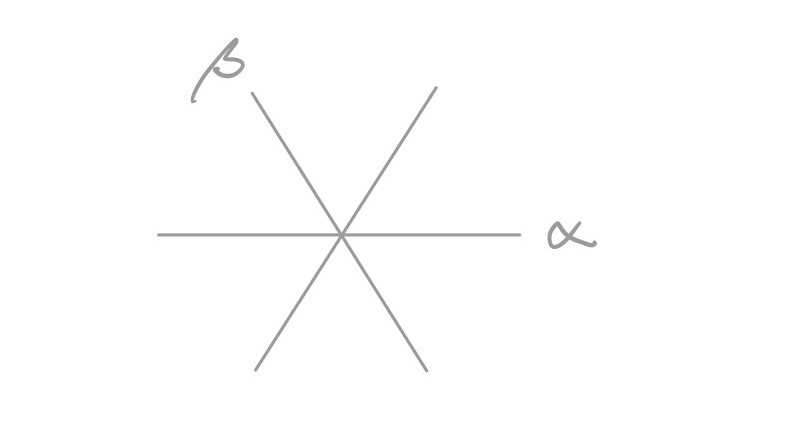
\includegraphics[scale=0.3]{A_2 root system.jpg}}

\noindent
We denote the admissible exponents $\eta, \nu$, where $\eta_{\alpha+\beta}, \eta_{-(\alpha+\beta)}=1$ and $\nu_{\alpha}, \nu_{-\alpha}=2$ and all other components zero, by

\centerline{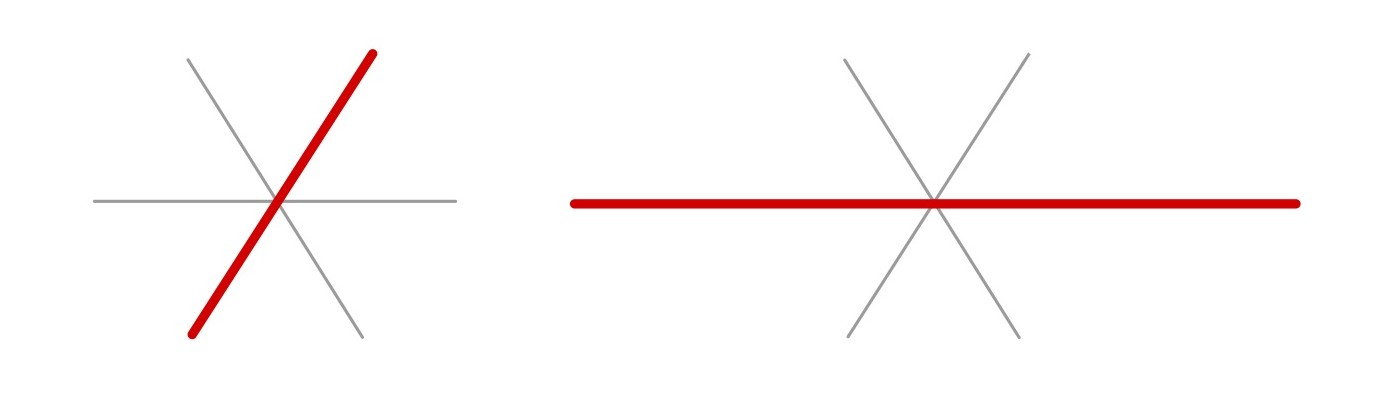
\includegraphics[scale=0.3]{A_2 diagram notation example.jpg}}

\noindent
We claim that the following is the complete set of simple admissible exponents for $A_2$ (it is straightforward to check these are all admissible and simple, though it is not obvious whether this is a complete set):

\centerline{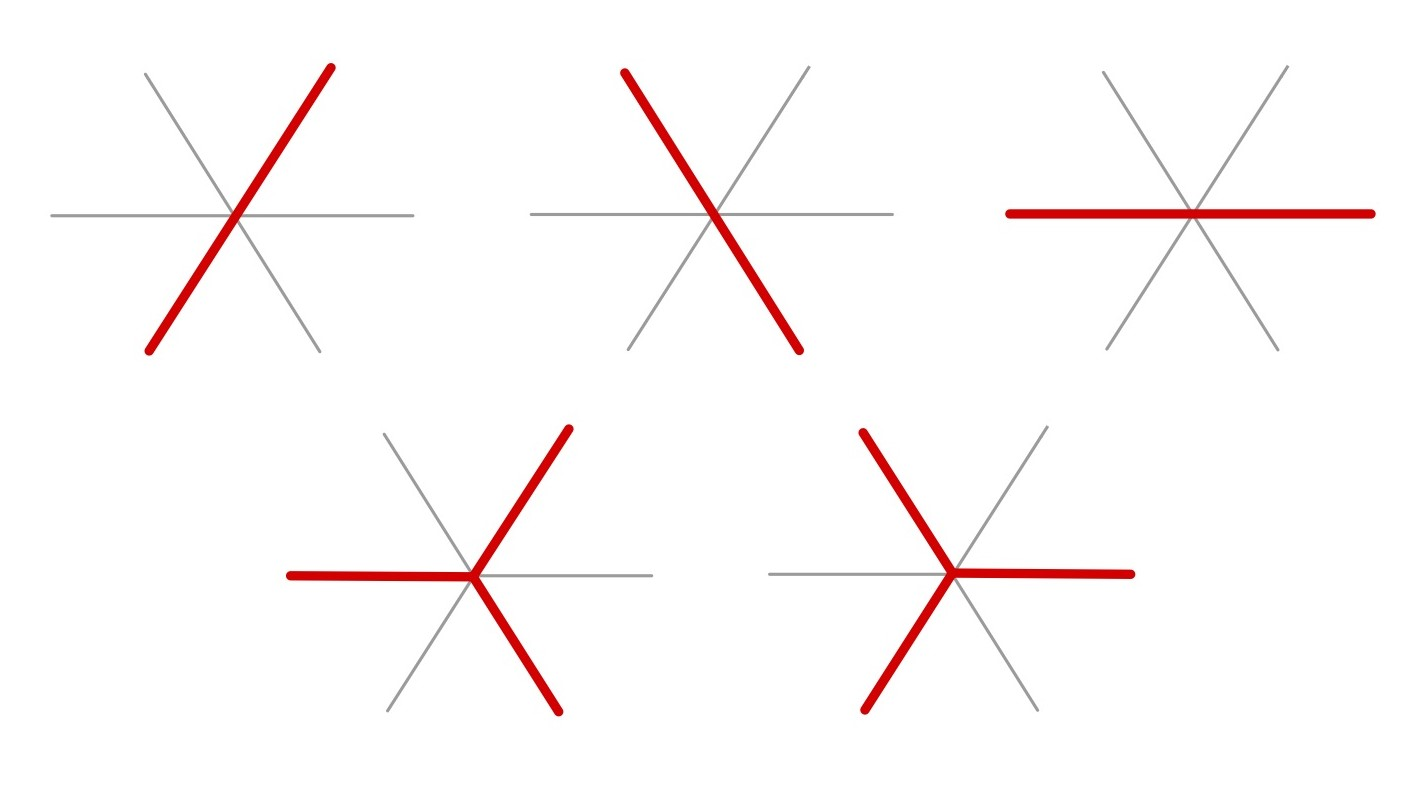
\includegraphics[scale=0.3]{A_2 simple admissibles.jpg}}

\noindent
If we consider the $C_2$ root system with the following choice of simple roots

\centerline{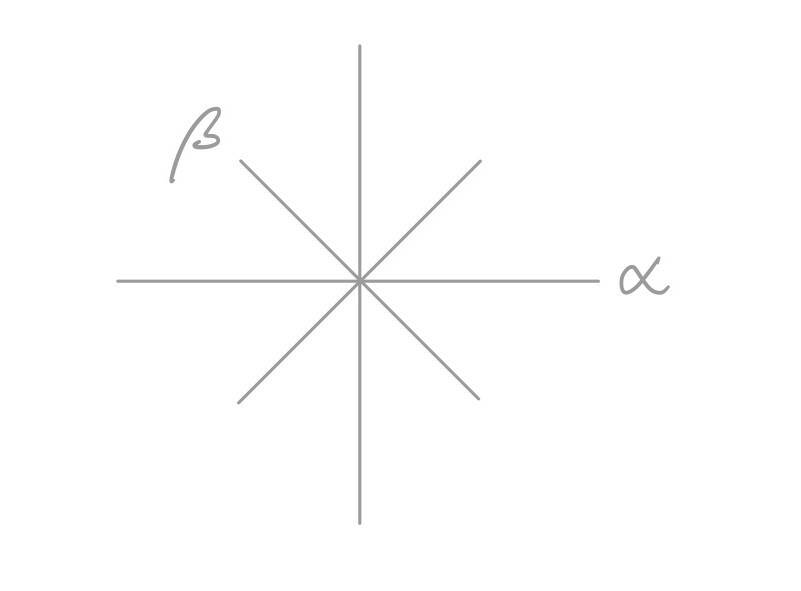
\includegraphics[scale=0.3]{C_2 root system.jpg}}

\noindent
Then we claim the following is the complete set of simple admissible exponents for $C_2$:

\centerline{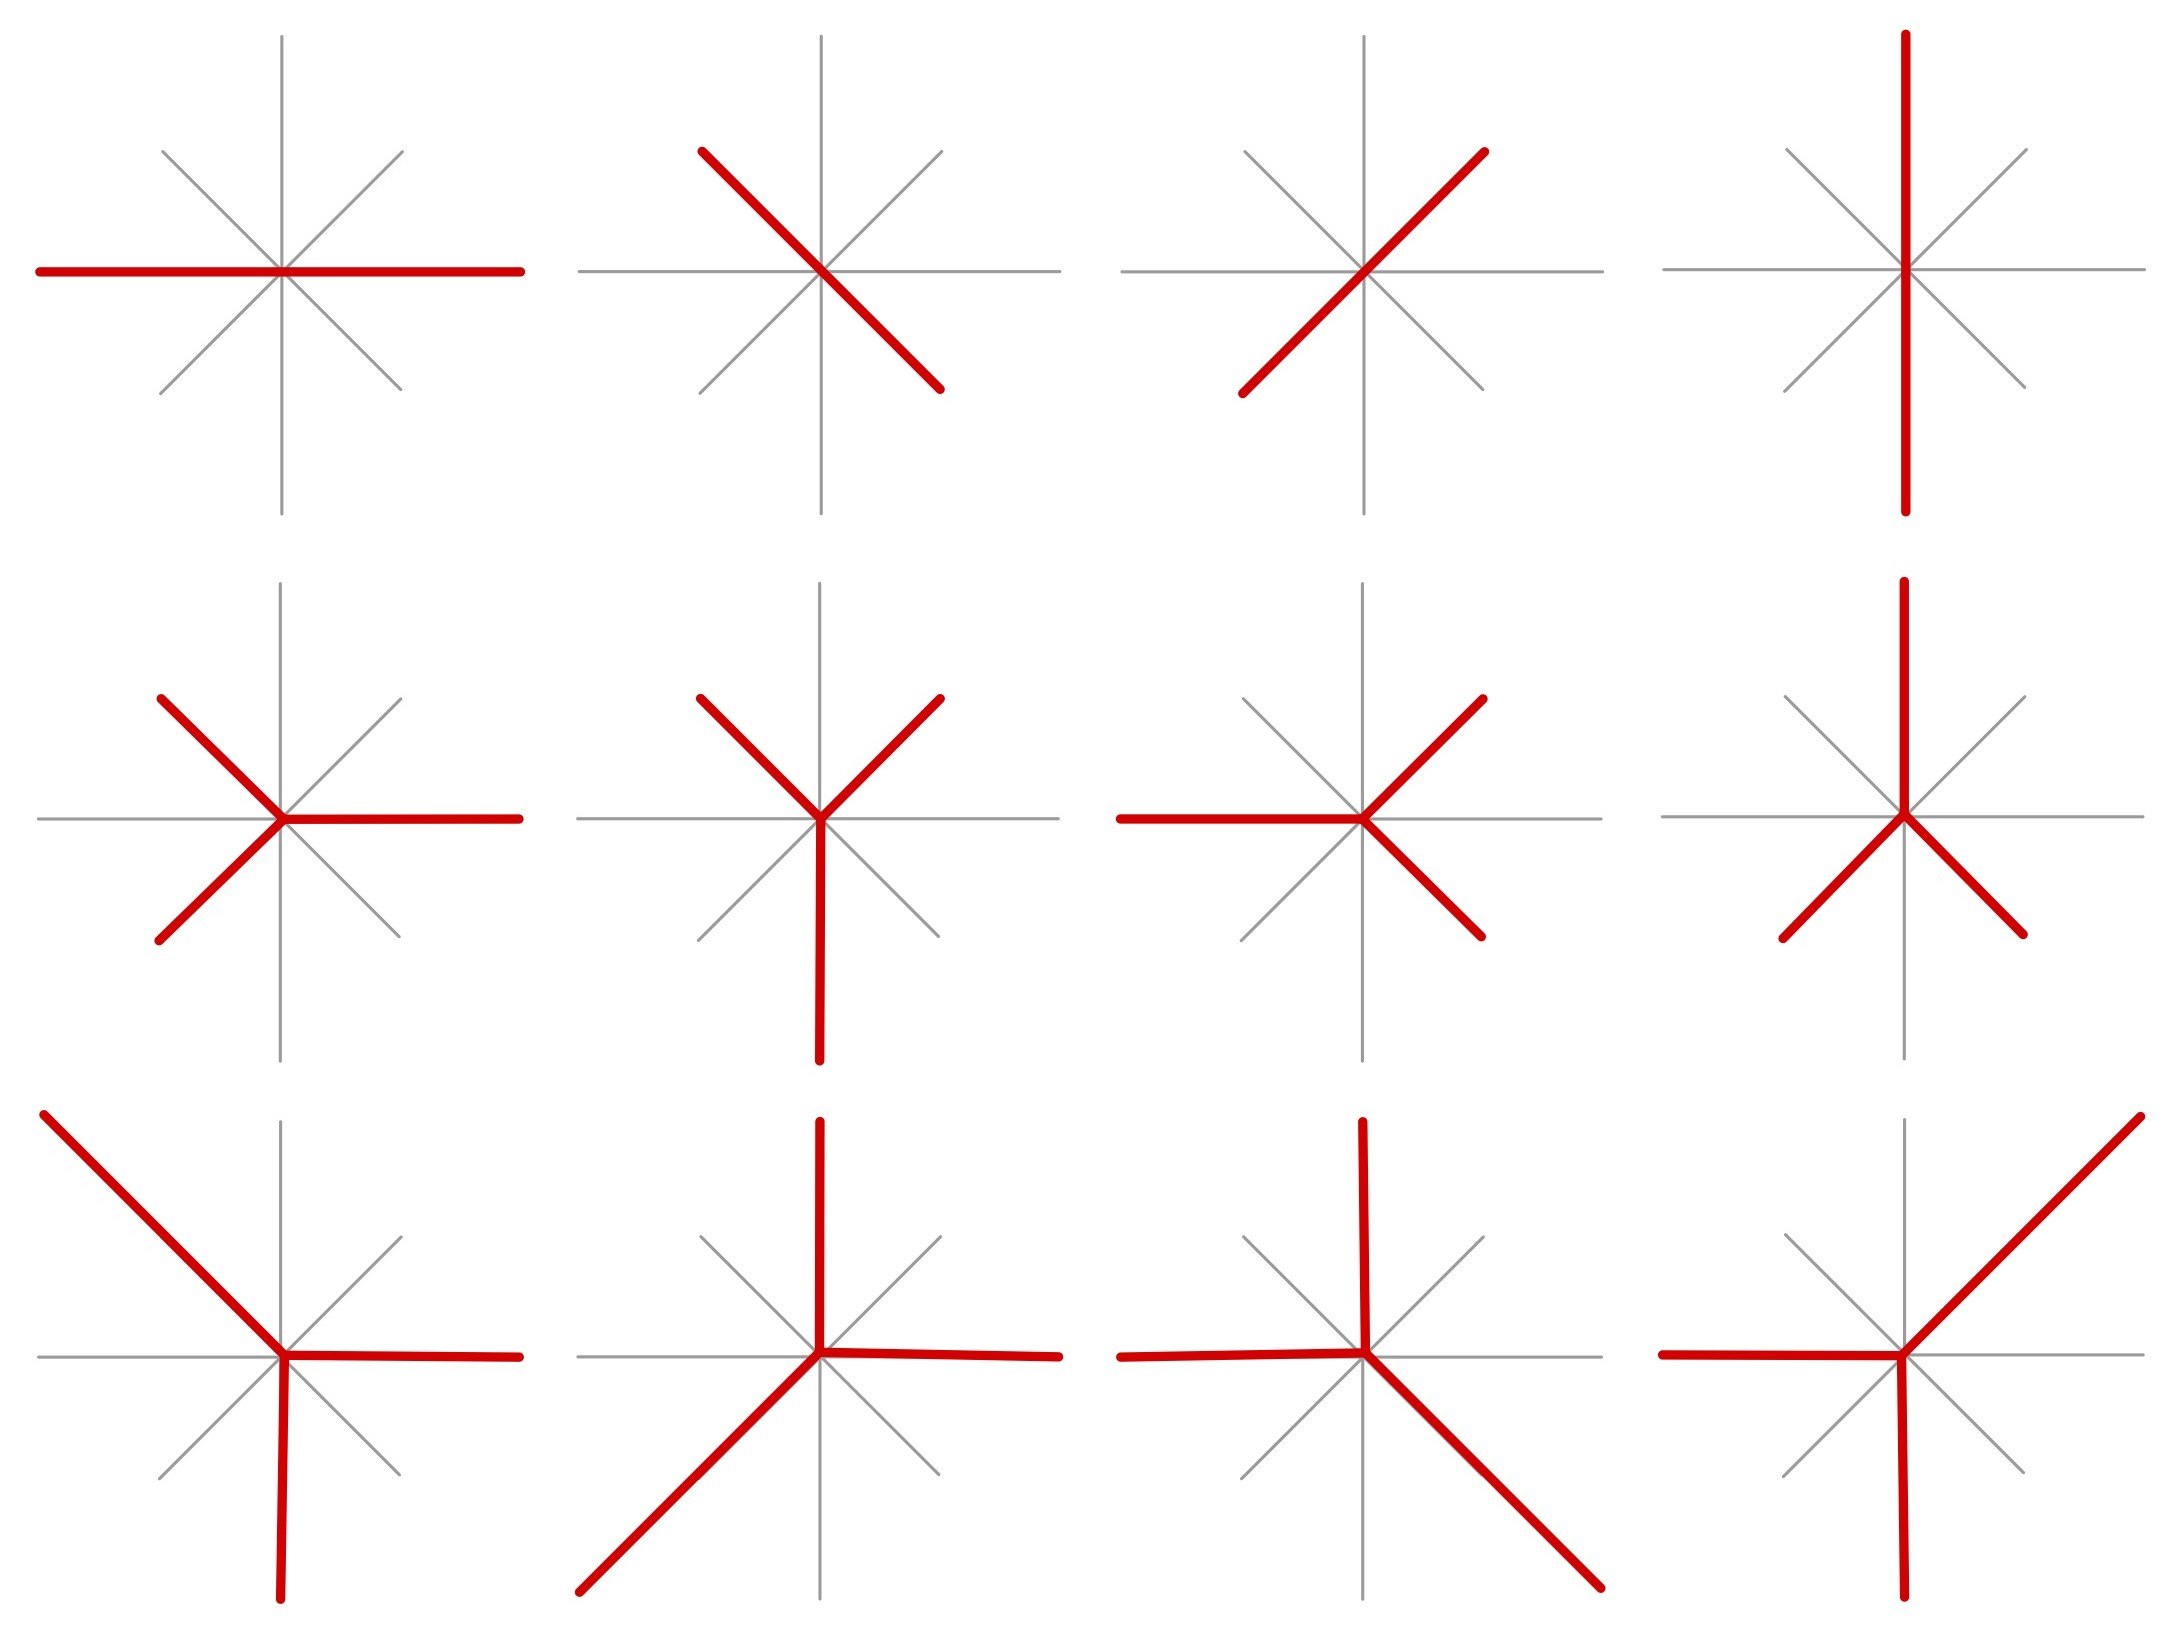
\includegraphics[scale=0.2]{C_2 simple admissibles.jpg}}

\end{moreexamples}

\emph{Finding all simple admissible exponents in the general case:}
Here is one way to find simple admissible exponents.
Let $\Delta$ be a choice of simple roots... (to discuss)


\begin{bibdiv}
\begin{biblist}
\bib{Hartshorne77}{book}{
   author={Hartshorne, Robin},
   title={Algebraic geometry},
   series={Graduate Texts in Mathematics},
   volume={No. 52},
   publisher={Springer-Verlag, New York-Heidelberg},
   date={1977},
   pages={xvi+496},
   isbn={0-387-90244-9},
   review={\MR{0463157}},
}

\bib{Humphreys72}{book}{
   author={Humphreys, James E.},
   title={Introduction to Lie algebras and representation theory},
   series={Graduate Texts in Mathematics},
   volume={Vol. 9},
   publisher={Springer-Verlag, New York-Berlin},
   date={1972},
   pages={xii+169},
   review={\MR{0323842}},
}

\end{biblist}
\end{bibdiv}

\end{document}